\documentclass{letter}
\usepackage{amsmath,amssymb,amsthm, graphicx,hyperref}
\begin{document}
\newtheorem{theorem}{Theorem}
\newtheorem{definition}{Definition}
\begin{center}
\LARGE \bf Strongly Bidirectional Self-Normalizing Neural Networks and Neural Networks All of Whose Derivatives are Bidrectional Self-Normalizing Neural Networks
\end{center}

\begin{center}
{\bf Abstract}

I give a stronger condition for bidirectional self-normalization that reduces the dependence on high-dimensional approximations in the method for bidirectional self-normalizing networks (BSNNs) of Lu et al. and construct BSNNs with the property that all their derivatives are BSNNs, allowing BSNNs to be applied to implicit representation learning. In implicit representation learning these methods can bring MSE between the image and the network output to below $10^{-8}$ in 400 iterations, which can be compared to the MSE of $10^{-5}$ achieved by Sitzman et al. using 10000 iterations.
\end{center}

\begin{center}
{\bf Background}
\end{center}

Sitzman et al., in {\it Implicit Neural Representations With Periodic Activation Functions} propose the use of periodic activation functions, specifically the use of the sine in the fitting of neural networks to, for example, images and signed distance functions. They prove that if the weights are uniformly distributed in $[-c,c]$ where $c=\sqrt{6/f}$ where $f$ is the fan in, then the pre-activations are always standard normal distributed irrespective of the depth of the network. Most importantly, the derivatives of these networks are networks of the same type (SIRENs), ensuring that these guarantees are applicable also to derivatives of networks of this type.

However, this provides no guarantees about the derivatives with respect to any parameter.

Lu et al., in {\it Bidirectional Self-Normalizing Neural Networks} prove a similar result: provided that the layers are orthogonal linear transformations that are uniformly distributed on the orthogonal group in the Haar sense followed by activation functions that are Gaussian-Poincaré normalized, meaning that the activation function $f$ satisfies $\mathbb{E}[f(Z)^2]=1$ and $\mathbb{E}[f'(Z)^2]=1$ where $Z$ is the standard normal distribution, $f$ and its derivative are Lipschitz continuous, and the input vector is thin-shell concentrated in the sense that for all $\epsilon>0$ $\mathbb{P}\left\{|\frac{1}{n}\|x\|_2^2-1|>\epsilon\right\}\rightarrow 0$ as $n\rightarrow \infty$ then the squared magnitude of the input to each layer is $n$ and the magnitude of the derivative of any loss function $E$ with respect to the input to any layer is the same provided that the layers are wide.

The guarantee that a thin-shell concentrated vector has its norm preserved under forward propagation in a BSNN is comparable to the guarantee that in a SIREN the pre-activations are standard normal distributed, but that the derivative of a loss function with respect to the input to any layer always has the same magnitude is an additional guarantee, which when taken together with the first becomes a much stronger assurance with regard to the trainability of deep BSNNs.

\begin{center}
{\bf Motivation}
\end{center}

In order to use BSNNs for the the same purpose of SIRENs we would have to construct BSNNs all of whose derivatives were BSNNs, specifically we would have to find differentiable functions which are Lipschitz continuous, whose first derivatives were Lipschitz continuous and which have the property that $E[f^{(n)}(Z)]=1$ for all $n$.

In a BSNN of some fixed finite width the pre-activations are uniformly distributed on the sphere with radius equal to the square root of the dimension, which in high dimension in a certain sense closely approximates the normal distribution so that the guarantees of Lu et al. can be obtained about the distribution of the activations even though the condition they impose is on the expectation of the activation function and its derivatives applied  to a standard normal distributed random variable. I propose a stronger condition, that $E[f(W)^2]=E[f'(W)^2]=1$ for all distributions $W$ such that $W \sim -W$. This will be assured if $f(x)^2-1$ and $f'(x)^2-1$ are odd functions.

\begin{definition}[Strong BSNN]
A neural network is said to be a strong BSNN if it has orthogonal weight matrices that are uniformly distributed in the Haar sense and the activation is differentiable, Lipschitz continuous with Lipschitz continuous derivative and has the property that $f(x)^2-1$ and $f'(x)^2-1$ are odd functions.
\end{definition}

We will be concerned with two problems: finding BSNNs all whose derivatives are BSNNs and characterizing the strong BSNNs.

\begin{center}
{\bf Characterization of strong BSNNs}
\end{center}

\begin{theorem}
If $f$ is the activation function of a strong BSNN then there is an even function $w$ taking values in $\{1,-1\}$ such that $f(x)^2-1=\sin(2\int_0^x w(s)ds)$.
\end{theorem}

\begin{proof}
Let $u(x)=f(x)^2-1$ and $v(x)=f'(x)^2-1$, then these are odd functions.

Since $v$ is odd $v(x)=-v(-x)$, i.e. $f'(x)^2-1 = -(f'(-x)^2-1)$ so that $f'(x)^2+f'(-x)^2=2$.

Also, $u'(x)=2f(x)f'(x)$ so that $u'(x)^2=4f(x)^2f'(x)^2$. Because $u(x)=f(x)^2-1$ $f(x)^2=u(x)+1$, so that we can write $u'(x)^2=4(u(x)+1)f'(x)^2$.

We now multiply $f'(x)^2 + f(-x)^2=2$ by $4(u(x)+1)f'(x)^2\cdot 4(u(-x)+1)f'(-x)^2$ and simplifying using the definition of $u'$ we obtain $4(u(-x)+1)u'(x)^2 + 4(u(-x)+1)^2=2\cdot 4(u(x)+1)\cdot 4(u(-x)+1)$.

Further simplifying and using that $u$ is an odd function we obtain $4u'(x)^2(u(x)+1-u(x)+1)=2\cdot 4^2(1-u(x)^2)$. Further simplifying we obtain $u'(x)^2=4(1-u(x)^2)$. Taking the square root we obtain $|u'(x)|=2\sqrt{1-u(x)^2}$.

Let $w(x)=\text{sgn}(u'(x))$. Since $w$ is the derivative of an odd function it is even.

Now $u'(x)=2w(x)\sqrt{1-u(x)^2}$, consequently $\frac{du}{\sqrt{1-u(x)^2}}=2w(x)dx$ and\newline $\arcsin(x)+C=2\int_0^x w(s)ds$ for some constant $C$. Thus $u(x)=\sin(2\int_0^x w(s)ds - C)$. Because $u$ is odd it is necessary that $u(0)=0$ and thus that $C=\pi\cdot n$ and we may take $C=0$ and absorb the sign into $w$ as $\sin(x + \pi)=-\sin(x)$ for all $x$.
\end{proof}

\begin{theorem}
Let be $w(x)$ an even function taking values in $\{1,-1\}$, then for any function $s(x)$ taking values in $\{1,-1\}$ such that $s(x)\sqrt{2}\sin(\int_0^xw(s)ds+\pi/4)$ is differentiable, Lipschitz and has Lipschitz derivative $s(x)\sqrt{2}\sin(\int_0^xw(s)ds+\pi/4)$ is the activation function of a strong BSNN.
\end{theorem}

The simplest of these activation functions is obtained with $w(x)=1$, $s(x)=1$ giving $f(x)=\sqrt{2}\sin(x+\pi/4)$. In this cases it is easy to see that $f(x)$ is a strong BSNN:

$\sqrt{2}\sin(x+\pi/4)=\sin(x)+\cos(x)$, thus $(\sin(x) + \cos(x))^2 = \sin(x)^2 + 2\sin(x)\cos(x) + \cos(x)^2 = 1 + 2\sin(2x)$. Consequently $\mathbb{E}[f(W)^2]=1 + \mathbb{E}[2\sin(W)\cos(W)]$ and $2\sin(x)\cos(x)$ is an odd function of $x$. The derivative is $\cos(x)-sin(x)$ and the computation splits the same way: $(\cos(x) - \sin(x))^2 = \cos(x)^2 - 2\cos(x)\sin(x) + \sin(x)^2=1 - \cos(x)\sin(x)$. Consequently $\mathbb{E}[f'(W)^2]= 1 - \mathbb{E}[2\cos(W)\sin(W)]=1$, again due to that $2\cos(x)\sin(x)$ is an odd function.

%Let $X$ be a random variable representing the pre-activations of a layer. If $\mathbb{E}%[f(X)^2]$ were not equal to one, then the activations $f(X)$ could not like on the sphere with . That $f$ is Gaussian-Poincaré normalized ensures that $\mathbb{E}[f(Z)]=1$ where $Z$ is the standard normal distribution, but $Z$ is only assured to be close to the standard normal distribution when the network is wide. However, $X$ is uniformly distributed on the sphere with radius equal to square root of the dimension. As the dimension increases this distribution becomes approximately standard normal distributed, but it straightforward that well before the dimensionality has grown so large that this is the case the distribution will be symmetric about zero, i.e. $X \sim -X$.

%If $f$ had the property that $f(x)^2-1$ was an odd function of $x$ this would ensure that $\mathbb{E}[f(X)^2]=1$ for any distribution $X$ such that $X\sim -X$.

%Similarly, if $\mathbb{E}[f'(X)]$ were not one, then $f'(X)$ would not be thin-shell concentrated, 

%is assured to be one due to the Gaussian-Poincaré normalization 

%If the pre-activations were standard-normal distributed then a Gaussian-Poincaré normalized activation function $f$ would ensure that $E[f(Z)^2]=1$ 

%These guarantees can only be obtained in the case of wide networks because thin-shell concentrated vectors are only approximately normal-distributed in high-dimensional spaces.

%Seeing as deeper networks generally have more representational power it is reasonable to hope that such deeper networks could be trained faster and have fewer parameters. Consequently it is of interest to construct deep BSNNs with the property that all their derivatives are BSNNs.

%Additionally, it is reasonable to hope to strengthen the guarantees of Lu et al. by requiring that the means $\mathbb{E}[f(W)^2]=1$ and $\mathbb{E}[f'(W)]=1$ where $W$ is a class of distributions containing the standard normal distribution.

\begin{center}
{\bf BSNNs all of whose derivatives are BSNNs}
\end{center}

In order to provide the strong guarantees ensured by theorems of Lu et al. also for derivatives of the network it is necessary to ensure that $E[f^{(n)}(Z)^2]=1$ for all $n$.

One such function is $e^{x-1}$, but another is the strong BSNN activation function $f(x)=\sqrt{2}\sin(x + \pi/4)$:

\begin{theorem}
Let $W$ and $-W$ have the same distribution and $f(x)=$\newline$=\sqrt{2}\sin(\frac{\pi}{4}+x)$, then $E[f^{(n)}(W)]=1$ for all $n$.
\end{theorem}

\begin{proof}
If $g$ is an odd function, i.e. $g(x)=-g(-x)$ then $\mathbb{E}[g(W)]=$\newline$=\mathbb{E}[-g(-W)]=-\mathbb{E}[g(-W)]$. Since $-W$ has the same distribution as $W$ it follows that $\mathbb{E}[g(W)]=-\mathbb{E}[g(W)]=0$.

Because $f''=-f$, it is sufficient to check that $\mathbb{E}[f(W)^2]=\mathbb{E}[f'(W)^2]=1$ to ensure that $\mathbb{E}[f^{(n)}(W)]=1$ for all $n$.

For the first equality $\mathbb{E}[(\sin(Z)+\cos(Z))^2]=E[\sin^2(Z)+2\sin(Z)\cos(Z)+\cos(Z)^2]=\mathbb{E}[1+\sin(2Z)]=1$, since the sine is odd. For second equality $\mathbb{E}[(\cos(Z)-\sin(Z))^2]=\mathbb{E}[\cos(Z)^2-2\sin(Z)\cos(Z)+\sin^2(Z)]=\mathbb{E}[1-\sin(2Z)]=1$, again since the sine is odd.
\end{proof}

When the activation function of a strong BSNN is infinitely differentiable its derivatives are in turn the activation functions of strong BSNNs, however, this only happens when $w$ is constant, i.e. when $w(x)=1$ or $w(x)=-1$. This corresponds to the activation functions $\sqrt{2}\sin(x + \pi/4)$ and $\sqrt{2}\cos(x + \pi/4)$.

\begin{center}
{\bf Positional Encoders}
\end{center}

We now have a concrete class of neural networks that can be trained: networks with linear layers of orthogonal linear transformations followed by this special sine or cosine activation function but, with the pre-condition that input vectors have squared magnitude equal to the square root of their dimension. This, and providing a good positional encoding, is the task of the positional encoder.

Mildenhall et al. in their paper {\it NeRF: Representing Scenes as Neural Radiance Fields for View Synthesis} describe a positional encoder assigning to each co-ordinate the vector $(\sin(2^0\pi p),\cos(2^0\pi p),...,\sin(2^{L-1}\pi p),\cos(2^{L-1}\pi p))$ where $p$ is the co-ordinate. These vectors have squared magnitude equal to one half their dimension, and by scaling them by $\sqrt{2}$ we would have a vector of the kind we need.

This method was originally applied to five-dimensional input, but when applied to two-dimensional input it introduces obvious patterns, likely present also in five dimensions, in the form of correlations between pixels along lines where one co-ordinate is constant.

These patterns can be removed by a slight modification of the encoder of Mildenhall et al.: taking the input co-ordinate pair $(x,y)^T$ we construct two additional co-ordinate pairs by rotating co-ordinate pair by one third and two-thirds a turn, to obtain two more $D_{2\pi/3}(x,y)^T$, $D_{4\pi/3}(x,y)^T$ where $D_\theta$ denotes a rotation in the x-y plane by $\theta$, and applying the encoder of Mildenhall et al. to each and concatenating the three outputs. Use of this positional encoder avoids line artifacts early in the network fitting and can be seen to improve final mean squared error.

\begin{center}
{\bf Application to Fitting of Images}
\end{center}

Networks of this type, when used with the improved positional encoder can bring MSE between the image and the network output to below $10^{-6}$ in around 100 iterations and to below $10^{-8}$ in around 400 iterations, compared to the $10^{-5}$ achieved by Sitzman et al. in their paper, which required 10000 iterations and 90 minutes on reasonably powerful GPU.

Below are plots of PSNR's, which in this case are $-10\log_{10}(\text{MSE})$ during two training runs, the first is a training run in which the learning rate is reduced aggressively and the second involves less aggressive learning rate reduction.

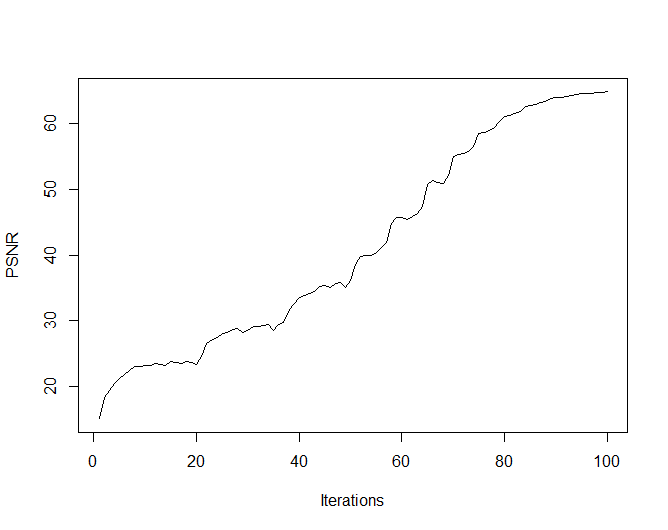
\includegraphics[scale=0.4]{PSNR-with-aggressive-training.png} 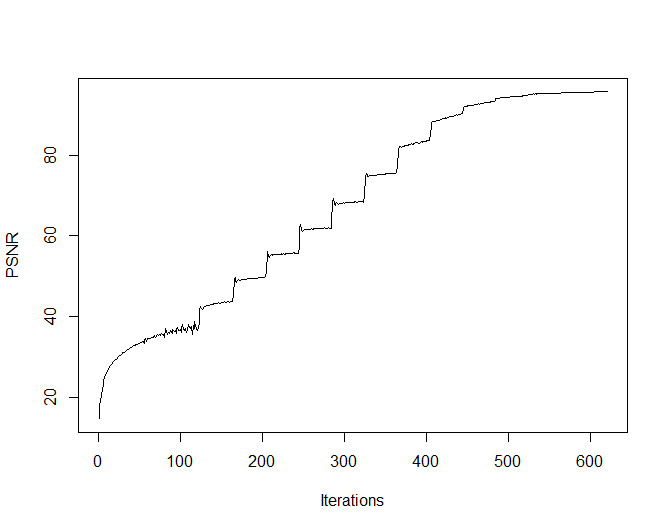
\includegraphics[scale=0.4]{PSNR-with-less-aggressive-training.png}

\begin{center}
{\bf Source Code and Video}
\end{center}

Source code for the experiments and a video showing the fitting process can be found on \href{https://github.com/mlaang/Neural-Networks--All-of-Whose-Derivatives-are-Self-Normalizing-Neural-Networks}{https://github.com/mlaang/Neural-Networks--All-of-Whose-Derivatives-are-Self-Normalizing-Neural-Networks}. The video can also be viewed directly on \href{https://www.youtube.com/watch?v=XYz6ayaKG_g}{https://www.youtube.com/watch?v=XYz6ayaKG\_g}.


\end{document}